공학에서 측정된 데이터를 사용하여 물리적 모델 혹은 요소들을 추정하는 경우가 대부분이다. 이 때 데이터는 연속적이기 보다는 이산적인 값으로 주어지는 경우가 많고, 이산적인 값 사이에 있는 임의의 점에서의 값을 추정해야 하는 경우가 있다. 또한 복잡한 함수를 단순화된 모델로 만들어야 하는 경우도 있다. 이 경우 임의의 수의 특정한 점들에서 그 함수값을 추적하고, 이들 계산값과 보간법을 이용하여 보다 간단한 형태의 함수로 표현할 수 있다. 이와 같은 응용들을 모두 일컬어 곡선적합(curve fitting)이라고 한다.

곡선적합은 데이터와 관련된 오차의 크기에 따라서 접근방법이 두 가지로 구별된다. 첫 번째 방법은 데이터가 상당한 크기의 오차 또는 "노이즈(noise)"를 내포하고 있을 경우로 데이터의 일반적인 경향을 나타내는 하나의 곡선을 유도해 내는 방법이다. 이 경우, 각각의 데이터값은 정확하지 않을 수 있기 때문에 유도되는 곡선이 모든 데이터점들을 통과하도록 노력할 필요는 없으나, 유도되는 곡선은 각 데이터점들의 경향을 따르도록 결정하여야 한다. 이러한 방식으로 데이터의 경향을 적절하게 표현하는 한 가지 방법으로 최소제곱회귀분석(least-square regression)이 있다. 두번째 방법은 데이터값들이 상당히 정확하여 각각의 데이터점들을 직접 통과하는 하나의 곡선, 또는 일련의 곡선들을 매끄럽게 연결하는 방법이다. 이 경우의 데이터는 보통 도표에 있는 값들로서, 예를 들면 온도의 함수로 표현되는 물의 밀도에 대한 값, 또는 가스의 비열에 대한 값들을 말한다. 값이 알려진 두 점들 사이에 있는 임의의 점에서 함수값을 추정하는 방법을 보간법(interpolation)이라고 한다.

\begin{figure}[!hbpt]
\centering
\subfigure[최소제곱회귀분석]{\includegraphics[keepaspectratio=true,width=0.3\linewidth]{MATLAB/chap11/pt5-1a.eps}}
\subfigure[선형보간]{\includegraphics[keepaspectratio=true,width=0.3\linewidth]{MATLAB/chap11/pt5-1b.eps}}
\subfigure[곡선보간]{\includegraphics[keepaspectratio=true,width=0.3\linewidth]{MATLAB/chap11/pt5-1c.eps}}
\label{fig:pt5-1}
\caption{10개의 점들을 최적의 곡선으로 보간하는 세가지 방법}
\end{figure}

경제공학에서 이율도표나, 열역학에서의 증기표 그리고 토목공학에서 응력변형도 곡선등과 같이 도표화된 데이터로부터 중간값을 결정하는 방식을 경험하였다. 비록 널리 사영되는 공학적 물성치들이 대부분이 도표화 혹은 공식화되어 있음에도 불구하고 많은 물성치들은 이러한 편리한 형태로 얻을 수 없다. 자신이 직접 데이터를 측정하거나, 예측관계식을 개발하여야 하는 특별한 경우와 같이 새로운 분야가 종종 발생된다. 실험데이터를 보간할 때는 경향분석(trend analysis)이나 가상실험(hypothesis testing)과 같은 두 가지 형태의 응용문제와 마주치게 된다.

경향분석은 예측을 하기 위하여 데이터의 형(pattern)을 분석하는 과정을 나타낸다. 데이터가 높은 정확도로 측정된 경우 보간다항식을 이용할 수 있으나, 정확도가 높지 않은 데이터는 보편적으로 최소제곱회귀분석이 사용된다.

실험적 곡선적합의 두 번째의 공학적 적용은 가상실험이다. 이것은 현존하는 수학적 모델과 측정된 데이터를 비교하는 것이다. 만약 모델의 계수들을 알지 못한다면, 관측된 데이터에 최적으로 적합한 계수들을 결정하여야 한다. 한편, 만약 모델 계수의 추정값이 이미 확보된 경우에는 관측된 값과 모델의 예측값을 서로 비교하여 모델의 적합성을 검사하는 것이 필요할 것이다. 이 때 대안으로 제시되는 모델과 비교되어 실험적인 관측에 근거한 "최적"인 모델이 선택된다.

\section{최소제곱회귀분석\\(Lest Square Regression)}
\subsection{통계학 기초}
공학적 연구 과정에서 어떤 특정한 양을 여러번 측정하였다고 가정하자. 

\begin{table}[!hbt]
\centering
\begin{tabular}{c|c|c|c|c|c}
\hline\hline
6.495&6.595&6.615&6.635&6.485&6.555\\
6.665&6.505&6.435&6.625&6.715&6.655\\
6.755&6.625&6.715&6.575&6.655&6.605\\
6.565&6.515&6.555&6.395&6.775&6.685\\
\hline\hline
\end{tabular}
\caption{철 구조물의 열팽창계수[$\times 10^{-6}\text{in}/(\text{in}\cdot^{\circ}\text{F})$]측정}
\label{tab:pt5-1}
\end{table}

예로 표\ref{tab:pt5-1}는 철 구조물(steel structure)의 열팽창계수에 관한 24개의 측정된 값들을 나타내고 있다. 표에 있는 값들을 보면 데이터는 최소 6.395로부터 최대 6.775의 범위 내에서 제한된 분량의 정보만을 제공하고 있다. 적절한 통계법을 이용하여 데이터를 요약하는 것으로 데이터 집합의 특수한 성질에 관하여 보다 많은 정보를 제공할 수 있는 추가적인 관찰 결과를 얻을 수 있다. 이러한 분석적인 통계법들은 (1) 데이터 분포의 중심위치 (2) 데이터 집합의 분산 정도등을 나타내는데 주로 사용된다.

가장 보편적인 통계값은 산술평균(arithmetic mean)이다. 어떤 표본의 산술평균($\bar{y}$)은 다음과 같이 각각의 데이터값($y_{i}$)들을 합하고, 이것을 데이터점의 수($n$)으로 나눈 것으로 정의된다.
\begin{equation}\label{eq:pt5-1}
\bar{y}=\frac{\sum y_{i}}{n}
\end{equation}

여기서 합(이후의 모든 합)은 $i=1$부터 $n$까지를 나타낸다.
또한, 가장 보편적인 표본의 분포도는 다음과 같이 정의되는 평균을 중심으로 하는 표준편차(standard deviation, $s_{y}$)이다.
\begin{equation}\label{eq:pt5-2}
s_{y}=\sqrt{\frac{S_{t}}{n-1}}
\end{equation}
여기서 $S_{t}$는 데이터점들과 평균 사이의 잔차를 제곱한 총합을 말한다. 즉 $S_{t}$는 다음과 같다.
\begin{equation}\label{eq:pt5-3}
S_{t}=\sum\left(y_{i}-\bar{y}\right)^{2}
\end{equation}
따라서 만약 개별적인 측정값들이 평균값 주변에 넓게 퍼져 있다면 $S_{t}$(결과적으로는 $s_{y}$)의 값은 커질 것이다. 만약에 측정값들이 모여 있다면 표준편차는 줄어든다. 분포는 표준편차의 제곱으로 다음과 같이 나타낼 수 있으며, 이것을 분산(variance, $s_{y}^2$)이라고 한다.
\begin{equation}\label{eq:pt5-4}
s_{y}^{2}=\frac{\sum\left(y_{i}-\bar{y}\right)^{2}}{n-1}
\end{equation}
여기서 식(\ref{eq:pt5-2})와 식(\ref{eq:pt5-4})에 있는 분모가 $(n-1)$인데 이것을 자유도(degree of freedom)이라고 한다. 따라서 $S_{t}$와 $s_{y}$는 $(n-1)$자유도에 기초를 두고 있다.
데이터 분포를 수치화하는 데 이용되는 통계값으로는 분산계수(coefficient of variation; c.v.)가 있으며, 이것은 평균에 대한 표준편차의 비율이다. 이 값은 정규화된 분포도를 다음과 같이 백분율의 형태로 나타내고 있다.
\begin{equation}\label{eq:pt5-5}
\text{c.v.}=\frac{s_{y}}{\bar{y}}\times 100
\end{equation}
\subsubsection{정규분포}
데이터가 평균값 주위에 분포되어 있는 형태가 있다. 히스토그램(histogram)은 데이터의 분포에 대한 간단한 시각적 표현을 제공해 주며, 측정값을 구간별로 분류해서 구성하게 된다. 이때 측정단위는 수평축에 나타내고 각 구간의 발생 빈도는 수직축에 나타낸다. 만약 많은 수의 데이터를 갖고 있을 경우 이러한 히스토그램은 매끄러운 곡선으로 근사화될 수가 있다.
\begin{figure}[!hbpt]
\centering
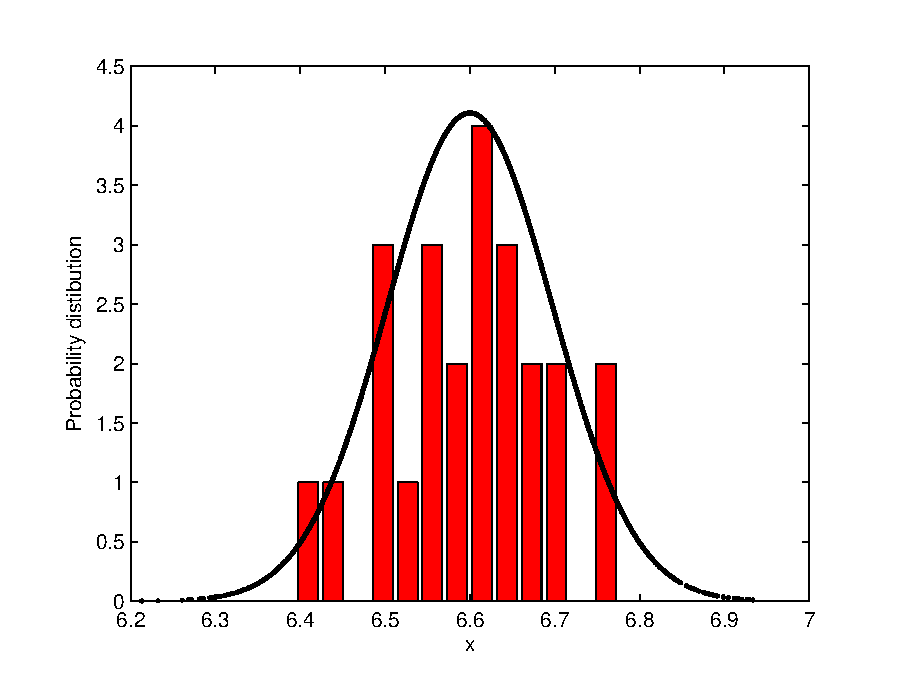
\includegraphics[keepaspectratio=true,width=0.6\linewidth]{MATLAB/chap11/dist.eps}
\label{fig:pt5-2}
\caption{정규분포}
\end{figure}
Figure~\ref{fig:pt5-2}에 나타낸 종 모양으로 된 대칭곡선은 이러한 근사화된 특성 곡선의 하나로써 정규분포(normal distribution)이라고 하며, 데이터점들의 수가 증가할 수록 히스토그램은 결국 이러한 정규분포에 접근하게 된다.

평균, 표준편차, 잔차의 제곱합 그리고 정규분포와 같은 개념들은 모두 공학문제와 큰 연관성을 갖고 있다. 매우 간단한 예로는 이들이 어떤 특정한 측정값에 대한 신뢰도를 정량화시키는데 사용될 수가 있다는 것이다. 만약 어떤 양이 정규적으로 분포되어 있다면 $\bar{y}-s_{y}$와 $\bar{y}+s_{y}$사이의 구간에는 전체 측정 개수의 약 68\%를 포함하게 된다. 같은 방식으로 아래의 식들과 같이 정량적인 방법으로 물리적인 양을 가늠할 수 있다.
\begin{align*}
\bar{y}-s_{y}\leq&\text{측정 개수의 }68\%\leq\bar{y}+s_{y}\\
\bar{y}-1.96s_{y}\leq&\text{측정 개수의 }95\%\leq\bar{y}+1.96s_{y}\\
\bar{y}-2.54s_{y}\leq&\text{측정 개수의 }99\%\leq\bar{y}+2.54s_{y}
\end{align*}
예를들어 Table~\ref{tab:pt5-1}에서와 같이 주어진 열팽창계수 데이터($\bar{y}=6.6$과 $s_{y}=0.097133$)에 대하여 우리는 약 95\%의 측정값들이 6.409619와 6.790381 사이에 존재한다고 할 수 있다. 만약에 어떤 사람이 7.35라는 값을 측정했다고 하면 우리는 그 측정값은 틀렸다고 의심하게 될 것이다. 이러한 측정값에 대한 신뢰도에 대한 평가는 다음절에서 다뤄진다.
\subsubsection{신뢰구간의 산출}
앞 절에서와 같이 통계의 주목적은 집단으로부터 제한적으로 추출된 표본을 이용하여 그 집단의 특성을 파악하는데 있다. 생산되는 모든 구조물용 강재의 열팽창계수를 측정한다는 것이 불가능함은 명백하다. Table~\ref{tab:pt5-1}와 같이 표본추출에 근거하여 전체 집단의 특성을 규명할 수가 있다.

제한된 표본으로부터 모르는 집단의 물성을 "추론"해야 하기 때문에 이러한 노력을 '통계적인 추론'이라고 한다. 통계적 추론의 결과는 보통 집단에 대한 인자들의 추정값으로 주어지기 때문에 이러한 과정을 '추정'이라고도 한다.

기호 $\bar{y}$ 및 $s_{y}$등은 표본의 평균 및 표준편차를 나타내고, 기호 $\mu$ 및 $\sigma$등은 집단의 평균 및 표준편차를 각각 나타낸다. 전자의 표현은 "산출(estimated)"된 평균 및 표준편차라고 하고, 후자의 표현은 종종 "참(true)"평균 및 표준편차라고 한다.

구간추정자(interval estimator)는 그 인자가 주어진 확률로 갖게 되는 값의 범위를 제시해 준다. 그러한 구간들은 한쪽이거나 양쪽인 것으로 설명될 수 있다. 한쪽 구간이라 함은 인자의 산출이 참값보다 작거나 또는 큰 신뢰도를 나타낸다. 반면에 양쪽 구간은 산출값이 항상 참값과 일치하게 되는 보다 일반적인 상황을 다루게 된다. 양쪽 구간이 보다 일반적이기 때문에 여기서는 이에 초점을 맞추어 설명한다.
양쪽 구간은 다음과 같이 기술 될 수 있다.
\begin{equation}
P\left\{L\leq\mu\leq U\right\}=1-\alpha
\end{equation}

\begin{figure}[!hbpt]
\centering
\includegraphics[keepaspectratio=true,width=0.6\linewidth]{MATLAB/chap11/norm.eps}
\label{fig:pt5-3}
\caption{양쪽 구간 신뢰도 범위}
\end{figure}
이것은 "$y$의 참평균 $\mu$가 $L$과 $U$ 사이의 구간에 놓일 수 있는 확률이 $(1-\alpha)$이다"라고 읽는다. 여기서 $\alpha$값을 유효수준(significant level)이라고 부르며, 따라서 신뢰구간 (confidence level)을 결정하는 문제는 $L$과 $U$를 구하는 것으로 축소된다. 필수조건은 아니지만 Figure~\ref{fig:pt5-3}과 같이 분포의 각 끝단 꼬리에 같은 크기로 $\alpha/2$씩 분포된 $\alpha$확률을 갖는 양쪽 구간을 관찰하는 것이 보편적이다.

$y$의 분포에 대한 참분산 $\sigma^2$을 알수 없지만 알고있다고 가정하면 표본의 평균 $\bar{y}$는 평균이 $\mu$이고 분산값이 $\sigma^2/n$인 정규분포로부터 얻어질 수가 있다. Figure~\ref{fig:pt5-3}에 설명된 문제에서 실제적인 평균 $\mu$를 모르고 있다. 그러므로 표본의 평균 $\bar{y}$와 관련해서 정규곡선이 정확하게 어디에 놓이게 되는지를 알지 못한다. 따라서 표준정규추정(standard normal estimate)로 새로운 값을 산출한다.
\begin{equation}\label{eq:pt5-6}
\bar{z}=\frac{\bar{y}-\mu}{\sigma/\sqrt{n}}
\end{equation}
이것은 $\bar{y}$와 $\mu$사이의 정규화된 거리를 나타낸다. 통계학적 이론에 의하면 이 값은 평균 0이고, 분산값이 1인 정규분포가 되어야 한다. 더욱이 $\bar{z}$가 Figure~\ref{fig:pt5-3}에서 면적표시가 되지 않은 영역에 떨어질 확률은 $(1-\alpha)$이어야 한다. 그러므로 $\alpha$의 확률로써 다음과 같은 표현이 가능하다.
\begin{align*}
\frac{\bar{y}-\mu}{\sigma/\sqrt{n}}&<-z_{\alpha/2}\\
\frac{\bar{y}-\mu}{\sigma/\sqrt{n}}&>z_{\alpha/2}
\end{align*}
$z_{\alpha/2}$는 표준정규 임의변수(standard normal random variable)이다. 이 값은 $(1-\alpha)$확률에 걸쳐 있으며, 평균을 전후해서 무차원화된 좌표축을 따라 측정된 거리를 나타낸다. 이 값은 각 상용프로그램으로도 구할 수 있다. 예를들어 $\alpha=0.05$ 즉 95\%의 확률에 걸치구간 $z_{\alpha/2}$는 약 1.96과 같다. 이런 결과는 확률 $(1-\alpha)$로써 다음과 같이 쓸 수 있다.
\begin{equation*}
L\leq\mu\leq U
\end{equation*}
여기서, $L$ 및 $U$는 각각 다음과 같이 정의된다.
\begin{align*}
L&=\bar{y}-\frac{\sigma}{\sqrt{n}}z_{\alpha/2}\\
U&=\bar{y}+\frac{\sigma}{\sqrt{n}}z_{\alpha/2}
\end{align*}
\subsection{선형회귀분석}
최소제곱 근사의 간단한 방법으로 관측치에 직선으로 적합시키는 것이다.
\begin{equation}\label{eq:15-1}
y=a_{0}+a_{1}x+e
\end{equation}
여기서, $a_{0}$는 절편(intercept), $a_{1}$는 기울기(slope)그리고 $e$는 관측값과 모델값의 차이로 오차(error)이다. 오차는 식(\ref{eq:15-1})를 변형하여
\begin{equation}
e=y-a_{0}-a_{1}x
\end{equation}
\subsubsection{최적적합을 위한 조건}
(1) 데이터를 통과하는 최적의 직선(best fit)을 구하는 방법은 모든 주어진 데이터에 대한 오차의 합을 최소화 시키는 것이다.
\begin{equation}\label{eq:15-2a}
\sum_{i=1}^{n}e_{i}=\sum_{i=1}^{n}(y_{i}-a_{0}-a_{1}x_{i})
\end{equation}
\framebox{문제점?}\\
(2) 오차의 절대값의 합을 최소화 하는 방법
\begin{equation}\label{eq:15-2b}
\sum_{i=1}^{n}\left|e_{i}\right|=\sum_{i=1}^{n}\left|y_{i}-a_{0}-a_{1}x_{i}\right|
\end{equation}
\framebox{문제점?}\\
(3) 최소-최대(minimax) 판별조건은 직선으로부터 떨어진 각 점들의 최대 변위가 최소가 되도록 선택하는 것이다.

위에서 언급한 방법들의 단점을 극복하기 위하여 측정된 $y$와 선형 모델을 이용하여 계산된 $y$사이의 잔차에 대한 제곱의 합을 최소화하는 방법이 고안됨.
\begin{align}
S_{r}&=\sum_{i=1}^{n}e_{i}^2\nonumber\\
&=\sum_{i=1}^{n}\left(y_{i,measured}-y_{i,model}\right)^2\nonumber\\
&=\sum_{i=1}^{n}\left(y_{i}-a_{0}-a_{1}x_{i}\right)^2\label{eq:15-3}
\end{align}
\subsubsection{직선의 최소제곱적합}
$a_{0}$와 $a_{1}$의 값을 결정하기 위하여 식(\ref{eq:15-3})은 각각의 계수에 대하여 편미분을 취한다.
\begin{align*}
\frac{\partial S_{r}}{\partial a_{0}}&=-2\sum\left(y_{i}-a_{0}-a_{1}x_{i}\right)\\
\frac{\partial S_{r}}{\partial a_{1}}&=-2\sum\left[\left(y_{i}-a_{0}-a_{1}x_{i}\right)x_{i}\right]\\
\sum y_{i}-\sum a_{0}-\sum a_{1}x_{i}&=0\\
\sum y_{i}x_{i}-\sum a_{0}x_{i}-\sum a_{1}x_{i}^{2}&=0
\end{align*}
$\sum a_{0}=na_{0}$이므로 이 식은 $a_{0}$과 $a_{1}$에 대한 2원 1차 연립방정식으로 주어진다.
\begin{align}
na_{0}+\left(\sum x_{i}\right)a_{1}&=\sum y_{i}\label{eq:15-4}\\
\left(\sum x_{i}\right)a_{0}+\left(\sum x_{i}^{2} \right)a_{1}&=\sum x_{i}y_{i}
\end{align}
이들을 정규 방정식(normal equation)이라고 한다. 이들을 연립방정식으로 풀면 $a_{1}$은 다음과 같이 된다.
\begin{equation}
a_{1}=\frac{n\sum x_{i}y_{i}-\sum x_{i}\sum y_{i}}{n\sum x_{i}^{2}-\left(\sum x_{i}\right)^{2}}
\end{equation}
이 결과를 식(\ref{eq:15-4})에 대입해서 $a_{0}$를 구하면
\begin{equation}
a_{0}=\bar{y}-a_{1}\bar{x}
\end{equation}
여기서 $\bar{y}$와 $\bar{x}$는 각각 $y$와 $x$의 평균이다.
\subsubsection{선형회귀분석 오차의 정량화}
최소제곱법으로 얻은 직선은 점들의 경향을 나타내는 "최적"의 유일한 직선이라 할 수 있다. 잔차들이 계산되는 방식을 자세히 분석해보면 보간법의 여러 다른 성질들을 발견할 수 있다. 식(\ref{eq:15-3})에서 정의된 제곱합을 상기해보면
\begin{equation}\label{eq:15-8}
S_{r}=\sum_{i=1}^{n}e_{i}^{2}=\sum_{i=1}^{n}\left(y_{i}-a_{0}-a_{1}x_{i}\right)^{2}
\end{equation}
여기서 식(\ref{eq:pt5-3})과 식(\ref{eq:15-8})이 유사함을 보인다. 즉 (1) 데이터와 직선과의 차이는 데이터의 전체 범위에 걸쳐서 유사한 크기를 갖고, (2) 직선을 중심으로 한 데이터점들의 분포는 정규분포를 이룬다. 만약 이들 판별조건이 만족된다면 최소제곱회귀분석은 $a_{0}$과 $a_{1}$를 구하는 가장 좋은방법이라고 할 수 있다.(Draper and Smith, 1981). 이것을 "최대우도법칙(maximum likelihood principle)"이라 한다.
회귀분석직선에 대한 표준편차는 다음과 같이 결정된다.
\begin{equation}\label{eq:15-9}
s_{y/x}=\sqrt{\frac{S_{r}}{n-2}}
\end{equation}
식(\ref{eq:pt5-3})의 데이터의 표준편차와 오차의 제곱합 식(\ref{eq:15-8})을 이용하여 상대적인 오차로 정규화하면
\begin{equation}\label{eq:15-10}
r^{2}=\frac{S_{t}-S_{r}}{S_{t}}
\end{equation}
여기서, $r^{2}$를 결정계수(coefficient of determination), $r$을 상관계수(correlation coefficient)라 한다. $S_{r}=0$, $r=r^{2}=1$인 경우, 완전한 적합이므로 데이터는 회귀분석직선에 의하여 100\%만족한다. 컴퓨터 계산을 위해 식(\ref{eq:15-10})를 다음 식과 같이 사용하는 것이 편리하다.
\begin{equation}
r=\frac{n\sum x_{i}y_{i}-\left(\sum x_{i}\right)\left(\sum y_{i}\right)}{\sqrt{n\sum x_{i}^{2}-\left(\sum x_{i}\right)}\sqrt{n\sum y_{i}^{2} -\left(\sum y_{i}\right)^2}}
\end{equation}

\begin{algorithm}

\begin{algorithmic}
\Function{regression}{$x$,$y$,$n$,$a_1$,$a_0$,$s_{y/x}$,$r^2$}
\State $sumx=0$\; $sumxy=0$\; $st=0$\;
\State $sumy=0$\; $sumx2=0$\; $sr=0$\;
\For{$i=1$,$n$}
 \State $sumx=sumx+x_{i}$\;
 \State $sumy=sumy+y_{i}$\;
 \State $sumxy=symxy+x_{i}*y_{i}$\;
 \State $sumx2=sumx2+x_{i}*x_{i}$\;
\EndFor
\State $x_{m}=sumx/n$\;
\State $y_{m}=sumy/n$\;
\State $a_{1}=(n*sumxy-sumx*sumy)/(n*sumx2-sumx*sumx)$\;
\State $a_{0}=y_{m}-a_{1}*x_{m}$\;
\For{$i=1$,$n$}
 \State $S_{t}=S_{t}+(y_{i}-y_{m})^{2}$\;
 \State $S_{r}=S_{r}+(y_{i}-a_{1}x_{i}-a_{0})^{2}$\;
\EndFor
\State $s_{y/x}=\sqrt{S_{r}/(n-2)}$\;
\State $r^{2}=(S_{t}-S_{r})/S_{t}$\;
\State \Return $a_{1}$, $a_{0}$, $s_{y/x}$, $r^2$
\EndFunction
\end{algorithmic}
\caption{선형회귀분석 알고리즘}
\end{algorithm}
%\framebox{예제} \textbf{Newton-Raphson법 예제 ($\sqrt{2}$ 찾기)}\\
%
%\begin{equation}\label{eq:e15-1}
%v(t)=\frac{gm}{c}\left(1-e^{(-c/m)t}\right)
%\end{equation}
%
%\begin{equation}\label{eq:e15-3-1}
%v(t)=\frac{gm}{c}\left(\frac{t}{3.75+t}\right)
%\end{equation}
%
%\begin{table}[!hbt]
%\centering
%\begin{tabular}{c|c|c|c}
%\hline\hline
%&Measured $v$&Model-calculated&Model-calculated\\
%&$m/s$&$m/s$ [Eq.\ref{eq:e15-1}]&$m/s$ [Eq.\ref{eq:e15-3-1}]\\
%Time (s)&(a)&(b)&(c)\\
%\hline
%1&10.00&8.953&11.240\\
%2&16.30&16.405&18.520\\
%3&23.00&22.607&23.729\\
%4&27.50&27.769&27.556\\
%5&31.00&32.065&30.509\\
%6&35.60&35.641&32.855\\
%7&39.00&38.617&34.766\\
%8&41.50&41.095&36.351\\
%9&42.90&43.156&37.687\\
%10&45.00&44.872&38.829\\
%11&46.00&46.301&39.816\\
%12&45.50&47.490&40.678\\
%13&46.00&48.479&41.437\\
%14&49.00&49.303&42.110\\
%15&50.00&49.988&42.712\\
%\hline\hline
%\end{tabular}
%\caption{낙하하는 낙하산병에 대한 측정 및 계산 속도값들}
%\label{tab:pt5-1}
%\end{table}

\subsubsection{비선형 관계식의 선형화}
선형식으로 회귀분석 할 수 있는 비선형 방정식의 형태는 다음과 같은 지수모델로 변형할 수 있다.
\begin{equation}\label{eq:15-12}
y=\alpha_{1}e^{\beta_{1}x}
\end{equation}
여기서 $\alpha_{1}$, $\beta_{1}$은 상수이다. 이 모델은 공학의 여러분야에서 증가하는 양($\beta_{1}>0$), 또는 감소하는 양($\beta_{1}<0$)이 그 자신의 크기에 직접 비례하는 특성을 나타내는 모델이다. 예로 인구 증가모델, 또는 바사능 감소등이다. 또한 멱방정식형태를 예를 들 수 있다.
\begin{equation}\label{eq:15-13}
y=\alpha_{2}x^{\beta_{2}}
\end{equation}
여기서 $\alpha_{2}$, $\beta_{2}$은 상수이다. 또한 포화성장률 방정식(saturation-growth-rate equation)이 있다.
\begin{equation}\label{eq:15-14}
y=\alpha_{3}\frac{x}{\beta_{3}+x}
\end{equation}
여기서 $\alpha_{3}$, $\beta_{3}$은 상수이다. 이 모델은 제한된 조건하의 인구 성장모델이나 $x$가 증가함에 따라 성장이 정지 즉, 포화상태에 이르는 비선형관계식을 나타내고 있다. 이러한 방정식모델은 간단한 조작으로 선형화가 가능하기 때문에 단순 선형회귀분석으로 보간식을 구할 수 있다. 예를들어 식(\ref{eq:15-12})의 양반여 자연로그를 취하면,
\begin{align}
\ln y&=\ln\alpha_{1}+\beta_{1}x\ln e\nonumber\\
&=\ln\alpha_{1}+\beta_{1}x\label{eq:15-15}
\end{align}
따라서 $x$에 대한 $\ln y$의 그림은 $\beta_{1}$인 기울기와 $\ln \alpha_{1}$인 절편을 갖는다. 마찬가지로 식(\ref{eq:15-13})은 양변에 상용로그를 취해 선형화할 수 있다.
\begin{equation}\label{eq:15-16}
\log y=\beta_{2}\log x+\log \alpha_{2}
\end{equation}
식(\ref{eq:15-14})는 역수를 취하여 다음과 같이 선형화될 수 있다.
\begin{equation}\label{eq:15-17}
\frac{1}{y}=\frac{\beta_{3}}{\alpha_{3}}\frac{1}{x}+\frac{1}{\alpha_{3}}
\end{equation}
\framebox{예제} \textbf{멱 방정식의 선형화}\\
데이터의 $\log$변환을 이용하여 Table~\ref{tab:15-3}에 있는 데이터를 식(\ref{eq:15-13})으로 나타내어라.

\begin{table}[!hbt]
\centering
\begin{tabular}{c|l|l|l}
\hline\hline
$x$&$y$&$\log x$&$\log y$\\
\hline
1&0.5&0&-0.301\\
2&1.7&0.301&0.226\\
3&3.4&0.477&0.534\\
4&5.7&0.602&0.753\\
5&8.4&0.699&0.922\\
\hline\hline
\end{tabular}
\caption{멱방정식으로 적합되는 데이터}
\label{tab:15-3}
\end{table}

\subsubsection{다항식 회귀분석}
2차다항식의 모델 방정식
\begin{equation}
y=a_{0}+a_{1}x+a_{2}x^2+e
\end{equation}
잔차의 제곱합은 다음식과 같다.
\begin{equation}
S_{r}=\sum_{i=1}^{n}\left(y_{i}-a_{0}-a_{1}x_{i}-a_{2}x_{i}^{2}\right)^{2}
\end{equation}
각 미지계수에 대해 편미분을 수행하면,
\begin{align*}
\frac{\partial S_{r}}{\partial a_{0}}&=-2\sum\left(y_{i}-a_{0}-a_{1}x_{i}-a_{2}x_{i}^{2}\right)\\
\frac{\partial S_{r}}{\partial a_{1}}&=-2\sum x_{i}\left(y_{i}-a_{0}-a_{1}x_{i}-a_{2}x_{i}^{2}\right)\\
\frac{\partial S_{r}}{\partial a_{2}}&=-2\sum x_{i}^{2}\left(y_{i}-a_{0}-a_{1}x_{i}-a_{2}x_{i}^{2}\right)
\end{align*}
$S_{r}$이 최소값을 갖는 경우 값을 0으로 두고 정규방정식으로 정리할 수 있다.
\begin{align*}
na_{0}+\left(\sum x_{i}\right)a_{1}+\left(\sum x_{i}^{2}\right)a_{2}&=\sum y_{i}\\
\left(\sum x_{i}\right)a_{0}+\left(\sum x_{i}^{2}\right)a_{1}+\left(\sum x_{i}^{3}\right)a_{2}&=\sum x_{i}y_{i}\\
\left(\sum x_{i}^{2}\right)a_{0}+\left(\sum x_{i}^{3}\right)a_{1}+\left(\sum x_{i}^{4}\right)a_{2}&=\sum x_{i}^{2}y_{i}
\end{align*}
행렬로 표시하면 다음과 같다.
\begin{equation}
\begin{bmatrix}n&\sum x_{i}&\sum x_{i}^{2}\\\sum x_{i}&\sum x_{i}^{2}&\sum x_{i}^{3}\\\sum x_{i}^{2}&\sum x_{i}^{3}&\sum x_{i}^{4}\end{bmatrix}\begin{Bmatrix}a_{0}\\a_{1}\\a_{2}\end{Bmatrix}=\begin{Bmatrix}\sum y_{i}\\\sum x_{i}y_{i}\\\sum x_{i}^{2}y_{i}\end{Bmatrix}
\end{equation}
즉 2차 다항식을 이용한 선형회귀문제는 쉽게 $n$차 다항식으로 확장될 수 있다. 
$n$개의 데이터를 $m$차 다항식으로 적합을 시키는 과정을 행렬법으로 접근해보자. 우선 1차식의 경우
\begin{align*}
y_{1}&=a_{0}+a_{1}x_{1}+e_{1}\\
y_{2}&=a_{0}+a_{1}x_{2}+e_{2}\\
y_{3}&=a_{0}+a_{1}x_{3}+e_{3}\\
\vdots&=\vdots\\
y_{n}&=a_{0}+a_{1}x_{n}+e_{n}
\end{align*}
행렬식으로 작성하면
\begin{align}
\begin{Bmatrix}y_{1}\\y_{2}\\y_{3}\\\vdots\\y_{n}\end{Bmatrix}&=\begin{bmatrix}1&x_{1}\\1&x_{2}\\1&x_{3}\\\vdots&\vdots\\1&x_{n}\end{bmatrix}\begin{Bmatrix}a_{0}\\a_{1}\end{Bmatrix}+\begin{Bmatrix}e_{1}\\e_{2}\\e_{3}\\\vdots\\e_{n}\end{Bmatrix}\\
\mathbf{Y}&=\mathbf{z}\cdot\mathbf{A}+\mathbf{e}
\end{align}
$m$차 다항식의 경우
\begin{align}
\begin{Bmatrix}y_{1}\\y_{2}\\y_{3}\\\vdots\\y_{n}\end{Bmatrix}&=\begin{bmatrix}z_{11}&\cdots&z_{1m}\\\vdots&&\vdots\\z_{n1}&\cdots&z_{nm}\end{bmatrix}\begin{Bmatrix}a_{0}\\\vdots\\a_{m}\end{Bmatrix}+\begin{Bmatrix}e_{1}\\e_{2}\\e_{3}\\\vdots\\e_{n}\end{Bmatrix}\\
\mathbf{Y}&=\mathbf{z}\cdot\mathbf{A}+\mathbf{e}
\end{align}
잔차는
\begin{equation}
\mathbf{e}=\mathbf{Y}-\mathbf{z}\cdot\mathbf{A}
\end{equation}
잔차의 제곱합은
\begin{align}
S_{r}&=\mathbf{e}^{\top}\mathbf{e}\\
&=(\mathbf{Y}-\mathbf{z}\cdot\mathbf{A})^{\top}(\mathbf{Y}-\mathbf{z}\cdot\mathbf{A})\label{eq:reg-29}
\end{align}
잔차의 제곱합을 최소로하기 위해 편미분을 취하면,
\begin{equation}
\frac{\partial \{\mathbf{e}^{\top}\mathbf{e}\}}{\partial\mathbf{A}}=0
\end{equation}
결론적으로 벡터미분을 계산하여 구하면,
\begin{equation}\label{eq:reg-31}
\mathbf{A}=\left[\mathbf{z}^{\top}\mathbf{z}\right]^{-1}\mathbf{z}^{\top}\mathbf{Y}
\end{equation}
\fbox{
\begin{minipage}{\textwidth}
벡터미분\\
먼저 $x_{1}^{2}+x_{2}^{2}$를 벡터 $\begin{bmatrix}x_{1}&x_{2}\end{bmatrix}^{\top}$에 대해 미분을 하면 다음과 같은 $n\times1$벡터$\begin{bmatrix}2x_{1}&2x_{2}\end{bmatrix}^{\top}$가 만들어진다. $1\times m$행렬을 $n\times1$ 벡터로 미분하면 $n\times m$행렬이 만들어진다. 즉, scalar를 벡터에 대해 미분하면 벡터의 각 요소로 한번씩 scalar를 미분하여 요소가 생성되는 미분한 벡터와 크기가 같은 벡터가 만들어진다. $1\times m$행벡터를 $n\times 1$열벡터로 미분하면 $n\times m$행렬이 만들어진다.
\begin{align*}
\mathbf{A}&=\begin{bmatrix}x_{1}^{2}+x_{2}^{2}&2x_{1}&2x_{1}^{3}+x_{2}\end{bmatrix}\\
\mathbf{x}&=\begin{bmatrix}x_{1}\\x_{2}\end{bmatrix}\\
\frac{\partial\mathbf{A}}{\partial\mathbf{x}}&=\begin{bmatrix}2x_{1}&2&6x_{1}^{2}\\2x_{2}&0&1\end{bmatrix}
\end{align*}
따라서 벡터미분은 다음과 같은 성질을 갖는다.
\begin{itemize}
\item \begin{equation*}\frac{\partial\left(\mathbf{x}^{\top}\mathbf{A}\right)}{\partial\mathbf{x}}=\mathbf{A}\end{equation*}
\item \begin{equation*}\frac{\partial\left(\mathbf{Ax}\right)}{\partial\mathbf{x}}=\mathbf{A}^{\top}\end{equation*}
\item \begin{equation*} \frac{\partial\left(\mathbf{x}^{\top}\mathbf{Ax}\right)}{\partial\mathbf{x}}=\mathbf{Ax}+\mathbf{A}^{\top}\mathbf{x} \end{equation*}
\end{itemize}

백터미분을 통하여 식(\ref{eq:reg-31})을 구해보자 식(\ref{eq:reg-29})을 전개하면
\begin{align*}
\mathbf{e}^{\top}\mathbf{e}&=(\mathbf{Y}-\mathbf{z}\cdot\mathbf{A})^{\top}(\mathbf{Y}-\mathbf{z}\cdot\mathbf{A})\\
&=(\mathbf{Y}^{\top}-\mathbf{A}^{\top}\mathbf{z}^{\top})(\mathbf{Y}-\mathbf{z}\cdot\mathbf{A})\\
&=\mathbf{Y}^{\top}\mathbf{Y}-\mathbf{Y}^{\top}\mathbf{zA}-\mathbf{A}^{\top}\mathbf{z}^{\top}\mathbf{Y}+\mathbf{A}^{\top}\mathbf{z}^{\top}\mathbf{zA}\\
\end{align*}
즉, 식(\ref{eq:reg-31})은 다음 식의 전개를 통해 구할 수 있다.
\begin{align}
\frac{\partial\left\{\mathbf{e}^{\top}\mathbf{e}\right\}}{\partial\mathbf{A}}&=\frac{\left\{\mathbf{Y}^{\top}\mathbf{Y}-\mathbf{Y}^{\top}\mathbf{zA}-\mathbf{A}^{\top}\mathbf{z}^{\top}\mathbf{Y}+\mathbf{A}^{\top}\mathbf{z}^{\top}\mathbf{zA}\right\}}{\partial\mathbf{A}}\\
&=-\mathbf{z}^{\top}\mathbf{Y}-\mathbf{z}^{\top}\mathbf{Y}+\mathbf{z}^{\top}\mathbf{zA}+\mathbf{z}^{\top}\mathbf{zA}\\
&=-2\mathbf{z}^{\top}\mathbf{Y}+2\mathbf{z}^{\top}\mathbf{zA}\\
&=0\\
\therefore \mathbf{A}&=\left[\mathbf{z}^{\top}\mathbf{z}\right]^{-1}\mathbf{z}^{\top}\mathbf{Y}\label{eq:ref-final}
\end{align}
\end{minipage}
}
즉 다항식의 최소제곱회귀분석은 식(\ref{eq:ref-final})와 같은 대수선형방정식으로 간단하게 구할 수 있다.